%\documentclass[10.5pt,twocolumn]{jsarticle}
\documentclass[twocolumn]{jsarticle}
  \usepackage{sounin}
  \usepackage{graphicx}
  \usepackage[dvipdfmx]{color}
  \usepackage{url}
  \pagestyle{empty}



\title{
高3総合人間科テンプレートファイル\\ \vspace{5pt}
{\fontsize{10pt}{0cm}\gt-使いにくいmicrosoft IMEとともに-}}

\author{名大付 花子}
\date{}


\begin{document}
\begin{abstract}
{\fontsize{9pt}{0cm}\mc
各段落の最初の一文をつなぐと、要約文ができあがるようにする。現在についてという点で関心が集まっている。先行研究ではが明らかになっている一方でについてはまだわかっていない。そこで本研究においてを研究課題とし、という仮説の下に、を研究した。その結果が明らかになった。本研究にはに対し、という意義があり、今後が期待される。
}\end{abstract}
\maketitle

\part{研究課題について}
\section{研究の背景}
現在についてという点で関心が集まっている。先行研究ではが明らかになっている一方でについてはまだわかっていない。そこで本研究においてを研究課題とし、という仮説の下に、を研究した。その結果が明らかになった。本研究にはに対し、という意義があり、今後が期待される。

\section{先行研究}
現在についてという点で関心が集まっている。
Aとはである。
Aに関心が集まったのは頃である。その後(時系列順に経緯を書く)、Bという点で注目されるようになった。



\section{研究課題と仮説}
本研究では〜を明らかにしていく。
先行研究等の分析から〜という仮説を立てた。

\section{研究の目的と意義}
この研究によって、〜が明らかになると、〜の点において〜の向上が期待される。


\part{第一期調査結果と考察}
\section{調査テーマ}



\section{調査時期と方法}


\section{調査結果}


\section{考察}


\part{第二期調査結果と考察}
\section{調査テーマ}
本調査は〜をテーマとして行った。

\section{調査時期と方法}
n個の調査を行った。
〜については文献調査を平成〜年〜月〜日から〜月〜日にかけて行った。
また、〜については令和〜年〜月〜日に、〜を対象にアンケート調査を行った。

\section{調査結果}
〜の結果は以下の表の通りである。


\section{考察}
〜については〜であることが考えられる。
また、〜に関しては図\ref{fig:school0}であることがはっきりと読み取れる。
したがって〜であるということが言えるだろう。

\begin{figure}[h]
  \begin{tabular}{c}
     \begin{minipage}[t]{1\hsize}
       \begin{center}
         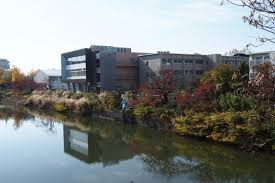
\includegraphics[clip,width=70mm,angle=0]{images/honko.jpg}
         \caption{本校図0}
         \label{fig:school0}
       \end{center}
     \end{minipage}
  \end{tabular}
\end{figure}

\part{結論}
\section{結論}
〜の結果、仮説が〜であるということが言える。
\section{今後の展望}
今回〜については明らかになったが(図\ref{fig:school1})、〜については完全に明らかにすることはできなかった。
今後は、〜に加え〜のような調査を行うことで、〜に関しても研究していきたいと考えている。

\begin{figure}[h]
  \begin{tabular}{cc}
     \begin{minipage}[t]{0.5\hsize}
       \begin{center}
         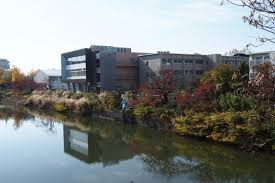
\includegraphics[clip,width=35mm,angle=0]{images/honko.jpg}
         \caption{本校図1}
         \label{fig:school1}
       \end{center}
     \end{minipage}
     \begin{minipage}[t]{0.5\hsize}
       \begin{center}
         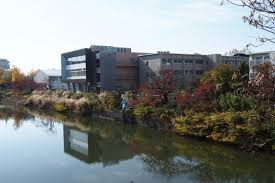
\includegraphics[clip,width=35mm,angle=0]{images/honko.jpg}
         \caption{本校図2}
         \label{fig:school2}
       \end{center}
     \end{minipage}
  \end{tabular}
\end{figure}


\begin{thebibliography}{10}
 \bibitem{platica} \url{大石隆司『理系数学の良問プラチカ数学I・A・II・B』(河合出版、2014年)}

\end{thebibliography}
\end{document}

